\section{Inferenčna statistika}

Metode sklepanja iz vzorca na populacijo. Uporabljamo teorijo verjetnosti, da ocenimo, koliko lahko zaupamo rezultatom, pridobljenim na verjetnostnem vzorcu.

\subsection*{Vzorčenje}

Je postopek izbire dela populacije, ki jo vključimo v raziskavo. Enote, ki so že izbrane pogosto ne vračamo v populacijo, če pa je velikost vzorca majhna, lahko to naredimo.

\subsubsection*{Metode vzorčenja}
\begin{itemize}
    \item \textbf{Verjetnostni vzorci}: Vsaka enota v populaciji ima znano neničelno verjetnost, da bo vključena v vzorec.
    \begin{itemize}
        \item \textit{Enostavno slučajno vzorčenje:} Vsaka enota ima enako in znano verjetnost izbire, ki ni enaka nič, notej so vsi možni vzorci enako verjetni. Primer: Z računalnikom naključno ustvarimo vzorec 100 dijakov, vpisanih na neko šolo v šolskem leti 2025/26 na podlagi seznama dijakov.
        \item \textit{Sistematično vzorčenje:} Iz vzorčnega okvirja vzamemo vsako $k$-to enoto. Vsaka enota ima enako verjetnost, da je izbrana v populacijo, toda vsi vzorci niso enako verjetni (npr. ne moremo hkrati izbrati četrte in pete enote, torej vzorčenje ni enostavno). Primer: Na podlagi seznama dijakov šole, ki je urejen po abecedi izberemo vsako deseto enoto. Naključno izberemo le prvo enoto npr. 2 in nadaljujemo z 12, 22, ....
        \item \textit{Stratificirano vzorčenje}: Popualcijo stratificiramo na podlagi vnaprej znanih informacij in nato izvedemo vzorčenje za vsak stratum posebej. Primer: Če ima šola 70\% dijakov in 30\% dijakinj, lahko vzamemo v vzorec enote proporcionalno glede na spol.
        \item \textit{Vzorčenje v skupinah}: Enote v populaciji so pogosto združene v skupinah, npr. učenci v razrede, razredi v šole, šole v države, itd. Tako lahko najprej izberemo vzorec skupin (npr. razredov) in naprej na temu vzorcu vzorčimo naprej. Primer: Na univerzi izberemo 5 od 15 programov in za vsakega od teh slučajno izberemo vzorec 100 študentov.
    \end{itemize}
    \item \textbf{Neverjetnostni vzorci}: Verjetnosti izbir ne moremo izračunati.
    \begin{itemize}
        \item \textit{Priložnostni vzorci}: Primer: Državljanom pošljemo 1 milijon vprašalnikov. (slabo)
        \item \textit{Ekspertna izbira}: Vzorec, ki naj bi bil reprezentativen izbere strokovnjak področja raziskave.
        \item \textit{Kvotno vzorčenje}: Primer: Med vzorčenjem nadziramo demografske značilnosti vzorca.
    \end{itemize}
    Nauk: Velikost vzorca ni vse. Pomembnejša je njegova reprezentativnost. V idealni situaciji bi uporabljali verjetnostno vzorčenje. Ko to ni možno, je kvotno vzorčenje boljša izbira kot priložnostno.\\
    Natančnost in točnost s sliko. (precision, accuracy)
\end{itemize}

\subsubsection*{Velikost vzorca}

Standardna napaka statistike je odvisna od velikosti vzorca.\\

Velikost vzorca za ocenjevanje aritmetične sredine navadno zahtevamo:

\[n>\left(\frac{z_{\frac{\alpha}{2}}\cdot\sigma}{E}\right)^2,\]

kjer $E$ označuje smiselno razliko med opazovanimi vrednostmi (navadno 1)

nekej nekej statistika

\subsection*{Intervali zaupanja}

Parametre lahko ocenimo točkovno ali z intervalom. Intervali zaupanja kažejo na točnost ocene in podajo informacijo o njeni zanesljivosti.\\
S tveganjem $\alpha$ lahko rečemo, da interval$(a,b)$ vsebuje parameter $\gamma$.

Slika normalne.

Širina intervala zaupanja je odvisna od:
\begin{itemize}
    \item \textit{Stopnje tveganja}: Višja je stopnja tveganja $\alpha$, ožji je interval
    \item \textit{Velikosti vzorca}: Večja je velikost vzorca $n$, ožji je interval.
\end{itemize}

\subsection*{Testiranje hipotez}

Znanstvena metoda:
\begin{enumerate}
    \item Opazovanje pojava
    \item Postavljanje raziskovalnih vprašanj
    \item Oblikovanje hipotez
    \item Zbiranje podatkov
    \item Sprejemanje hipotez in razvoj teorij in zakonitosti
\end{enumerate}

Primer: Raziskovalno vprašanje: Ali obstajajo razlike med spoloma v matematični anksioznosti?\\
Hipoteza: Ženske imajo več matematične anksionosti kot moški ($H_0: \mu_z - \mu_m >0$).

Opomba: Hipoteza je vedno trditev, ki jo lahko poskušamo zavrniti. Hipoteza ni potrjena in tehnično ni pravilno reči, da je hipoteza sprejeta. Hipotezo lahko ali zavrnemo ali ne zavrnemo.

Ničelno hipotezo $H_0$ lahko neposredno preverimo in če je zavrnjena, je alternativna hipoteza pravilna (to je običajno naši cilj)\\
Alternativno hipotezo $H_1$ preverimo le posredno: če ničelne hipoteze ne moremo zavrniti, ničelne hipoteze ne sprejmemo, ampak sklenemo, da ni dovolj podatkov, da bi rekli, ali je razlika statistično pomembna

Primer: Ničelna hipoteza: Med ženskami in moškimi ni razlike v sposobnosti večopravilnosti. Alternativna hipoteza: Obstajajo razlike v sposobnosti večopravilnosti med ženskami in moškimi (dvostranski test). Alternativna hipoteza: Ženske so boljše pri večopravilnosti kot moški (enostransko testiranje)

V statistiki ločimo med dvema vrstama napak, ki ju lahko naredimo pri testiranju hipotez:
\begin{itemize}
    \item \textbf{Napaka prve vrste ($\alpha$-napaka):} To je napaka, ki jo naredimo, ko zavrnemo ničelno hipotezo ($H_0$), čeprav je v resnici resnična. Gre torej za "lažno pozitivni" rezultat. Verjetnost, da se zgodi napaka prve vrste, imenujemo raven značilnosti $\alpha$, ki je običajno nastavljena na 0,05 ali 5 \%. To pomeni, da obstaja 5-odstotna možnost, da napačno zavrnemo resnično ničelno hipotezo.
    \item \textbf{Napaka druge vrste ($\beta$-napaka):} To je napaka, ki jo naredimo, ko ne zavrnemo ničelne hipoteze ($H_0$), čeprav je v resnici napačna. Gre za "lažno negativni" rezultat. Verjetnost, da se zgodi napaka druge vrste, označujemo z $\beta$. Komplement te verjetnosti $(1-\beta)$ predstavlja moč testa, ki je verjetnost, da bomo pravilno zavrnili napačno ničelno hipotezo.
\end{itemize}

V praksi se moramo zavedati, da je zmanjšanje verjetnosti ene vrste napake običajno povezano s povečanjem verjetnosti druge vrste napake, zato je pomembno, da testiranje hipotez izvedemo premišljeno in uravnotežimo tveganja za obe vrsti napak.


\subsection*{Stopnja značilnosti}

Izberemo največjo verjetnost $\alpha$ stopnjo, do katere smo pripravljeni tvegati napako tipa I. Običajno se odločimo za $5\%$ stopnjo značilnosti $(\alpha = 0.05)$ , lahko pa je tudi $1\%\  (\alpha = 0.01)$ ali nižja. Na podlagi izbranega $\alpha$ določimo kritično območje, kjer bo ničelna hipoteza zavrnjena. Pri tem upoštevamo, ali gre za dvostranski ali enostranski test

\begin{figure}[h]
    \centering
    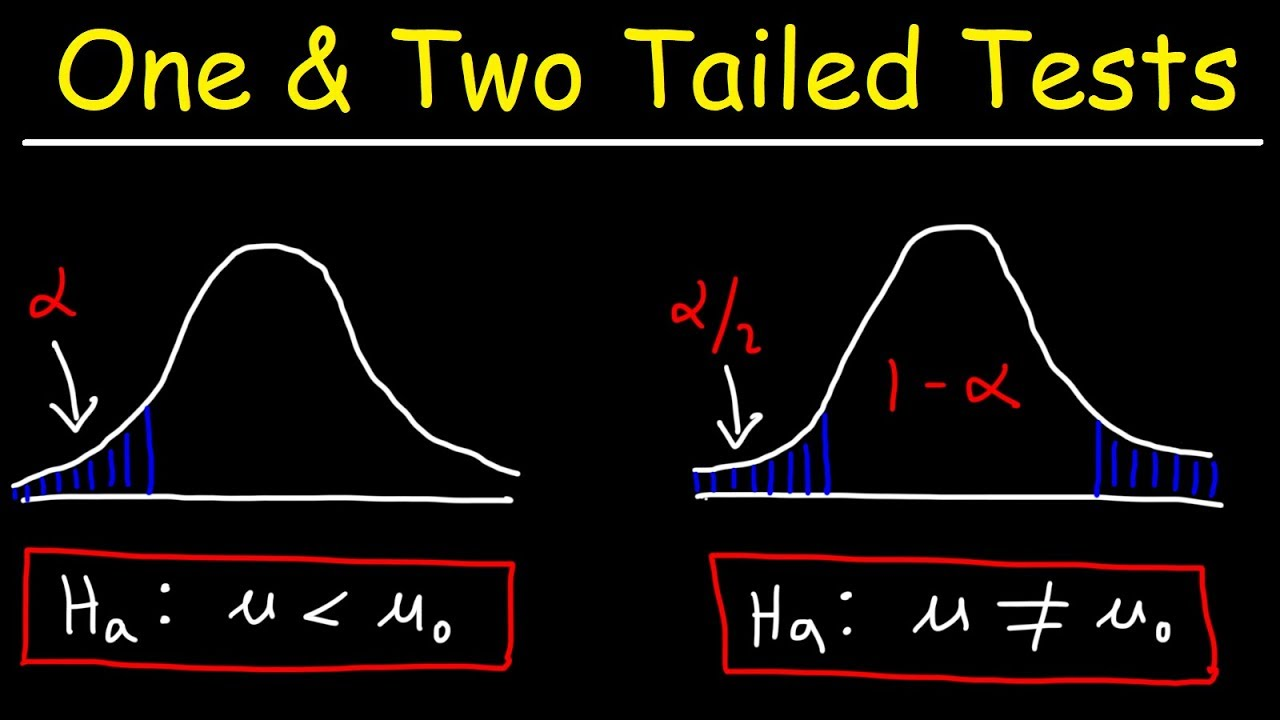
\includegraphics[width=\textwidth]{pictures/one_two_tail.jpg}
    \caption{This is a caption for the figure.}
    \label{fig:one_two_tail}
\end{figure}

\subsection*{Studentova $t$ porazdelitev}

\begin{figure}[h]
    \centering
    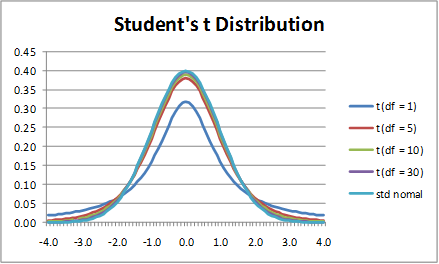
\includegraphics[width=\textwidth]{pictures/t_porazdelitev.png} % Replace 'example-image' with your image file name
    \caption{This is a caption for the figure.}
    \label{fig:t_porazdelitev}
\end{figure}

Razpršenost je odvisna od tako imenovanih prostostnih stopenj (\textit{angl. degrees of freedom}, $df$), ki so opredeljene kot velikost vzorca minus število parametrov populacije, ki jih je treba oceniti na podlagi vzorca.\\
Večji kot je vzorec, bližje je $t$ porazdelitev normalni $Z$ porazdelitvi

\subsection*{$T$ test za en vzorec}

Primerjava povprečja na vzorcu z določeno vrednostjo (npr. populacijskim parametrom ali nevtralno točko na lestvici)\\
\[t = \frac{mean-comparison}{standard error}\]
Predpostavke:
\begin{itemize}
\item Slučajno vzorčenje, neodvisni vzorci
\item Normalna porazdelitev podatkov (če je $N < 30$)
\end{itemize}

Primer: Ali se študenti pri preizkusu odrežejo bolje od naključja?\\
28 študentov je opravilo test s 100 vprašanji o besedilu, ki ga niso prebrali.\\
Vsako vprašanje je imelo 5 možnih odgovorov, zato bi pri povsem naključni izbiri pričakovali, da bo pravilno izbranih 20 postavk.\\
Vendar so v povprečju pravilno odgovorili na 46,57 vprašanj. S t-testom za en vzorec (angl. one-sample t-test) pokažemo, da so se študenti odrezali statistično značilno bolje od naključja $(M=46.57, t(27)=20.6, p < 0.001)$.

\begin{Vaje}{1}
    Izbrali smo vzorec šestnajstih otrok in jih stehtali. Določi interval zaupanja za pravo vrednost aritmetične sredine s $5\%$ tveganja.\\
    X: 35 37 29	26 31 32 28	40 27 33 33	34 31 30 29	38
\end{Vaje}
\begin{Vaje}{2}
Imamo podatke za vzorec učencev o tem, koliko ur tedensko porabijo za učenje doma. 78 jih je odgovorilo, da se pripravljajo na pouk 2 do 3 ure tedensko, 125 s jih uči 3 do 4 ure na teden, 103 se učijo vsak teden več kot 4 ure. Določi odstotek tistih učencev, ki tedensko posvečajo učenju najmanj časa in oceni ta odstotek v osnovni množici (z $1\%$ tveganjem).
\end{Vaje}
\begin{Vaje}{3}
Učitelja matematike zanima, ali je povprečno število točk njegovih učencev na preizkusu znanja višje od nacionalnega povprečja, ki je 75. Izračunajte vrednost $t$-statistike pri stopnji tveganja $5 \%$, določite kritično območje in sklepajte o rezultati za naslednje podatke:\\
Za sodelovanje v raziskavi je bil izbran vzorec 25 učencev.\\
Povprečna ocena iz matematičnega izpita v vzorcu je 80.\\
Standardni odklon v vzorcu je 6.
\end{Vaje}
\begin{Vaje}{4}
    Želimo določiti minimalno velikost vzorca za pilotno študijo novega izobraževalnega programa. Standardni odklon učinka programa na bralne sposobnosti je 3 točke. Želite imeti $95\%$ stopnjo zaupanja, da bo vaša ocena učinka natančna. Izračunajte minimalno velikost vzorca.
\end{Vaje}